\documentclass[12pt]{article}%
\usepackage{amsfonts}
\usepackage{fancyhdr}
\usepackage{comment}
\usepackage[a4paper, top=2.5cm, bottom=2.5cm, left=2.2cm, right=2.2cm]%
{geometry}
\usepackage{times}
\usepackage{amsmath}
%\usepackage{colorlinks,linkcolor=red}{hyperref}
\usepackage{changepage}
\usepackage{amssymb}
\usepackage{listings}
\usepackage{graphicx}%
%table
\usepackage{tabu}
\usepackage{booktabs}
\usepackage{threeparttable}
\usepackage{multirow}
\usepackage{url}


\setcounter{MaxMatrixCols}{30}
\newtheorem{theorem}{Theorem}
\newtheorem{acknowledgement}[theorem]{Acknowledgement}
\newtheorem{algorithm}[theorem]{Algorithm}
\newtheorem{axiom}{Axiom}
\newtheorem{case}[theorem]{Case}
\newtheorem{claim}[theorem]{Claim}
\newtheorem{conclusion}[theorem]{Conclusion}
\newtheorem{condition}[theorem]{Condition}
\newtheorem{conjecture}[theorem]{Conjecture}
\newtheorem{corollary}[theorem]{Corollary}
\newtheorem{criterion}[theorem]{Criterion}
\newtheorem{definition}[theorem]{Definition}
\newtheorem{example}[theorem]{Example}
\newtheorem{exercise}[theorem]{Exercise}
\newtheorem{lemma}[theorem]{Lemma}
\newtheorem{notation}[theorem]{Notation}
\newtheorem{problem}[theorem]{Problem}
\newtheorem{proposition}[theorem]{Proposition}
\newtheorem{remark}[theorem]{Remark}
\newtheorem{solution}[theorem]{Solution}
\newtheorem{summary}[theorem]{Summary}
\newenvironment{proof}[1][Proof]{\textbf{#1.} }{\ \rule{0.5em}{0.5em}}

\newcommand{\Q}{\mathbb{Q}}
\newcommand{\R}{\mathbb{R}}
\newcommand{\C}{\mathbb{C}}
\newcommand{\Z}{\mathbb{Z}}

\begin{document}

\title{SysEng5212 /EE 5370 Project:Automated Image Interpretation via ConvNets \& Recurrent Networks}
\author{Xiongming Dai}
\date{May 4,2018}
\maketitle


\section{Introduction}

A quick glance at an image is sufficient for a human to point out and describe an immense amount of details about the visual scene [3]. However, this remarkable ability has proven to be an elusive task for our visual recognition models. The majority of previous work in visual recognition has focused on labeling images with a fixed set of visual categories and great progress has been achieved in these endeavors [10]. However, while closed vocabularies of visual concepts constitute a convenient modeling assumption, they are vastly restrictive when compared to the enormous amount of rich descriptions that a human can compose.

Some pioneering approaches that address the challenge of generating image descriptions have been developed [6]. However, these models often rely on hard-coded visual concepts and sentence templates, which imposes limits on their variety. Moreover, the focus of these works has been on reducing complex visual scenes into a single sentence, which we consider to be an unnecessary restriction.

In this project, we strive to take a step towards the goal of generating dense descriptions of images (Figure 1). The primary challenge towards this goal is in the design of a model that is rich enough to simultaneously reason about contents of images and their representation in the domain of natural language. Additionally, the model should be free of assumptions about specific hard-coded templates, rules or categories and instead rely on learning from the training data. The second, practical challenge is that datasets of image captions are available in large quantities on the internet [7], but these descriptions multiplex mentions of several entities whose locations in the images are unknown.

\begin{figure}[t]
\begin{center}
%\fbox{\rule{0pt}{2in} \rule{0.9\linewidth}{0pt}}
   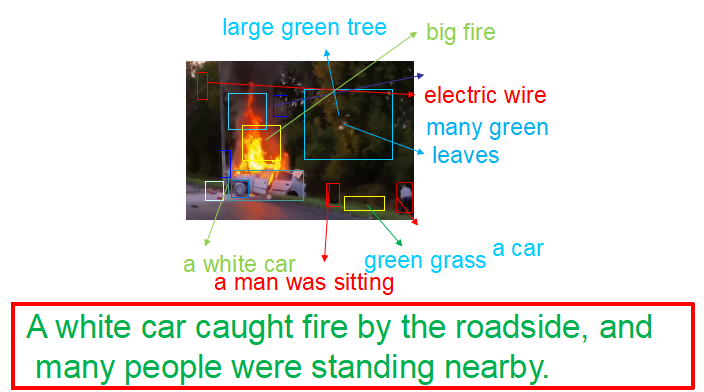
\includegraphics[width=0.8\linewidth]{p111.jpg}
\end{center}
   \caption{Motivation/Concept Figure: Our model treats language as a rich label space and generates descriptions of image regions.}
\label{fig:circle}
\end{figure}

Our core insight is that we can leverage these large image-sentence datasets by treating the sentences as weak labels, in which contiguous segments of words correspond to some particular, but unknown location in the image. Our approach is to infer these alignments and use them to learn  a generative model of descriptions. Concretely, our contributions are twofold:

We develop a deep neural network model  that  infers the latent alignment between segments of sentences and the region of the image that they describe. Our model associates the two modalities through a common, multimodal embedding space and a structured objective. We validate the effectiveness of this approach on image-sentence retrieval experiments in which we surpass the state-of-the-art.

We introduce a multimodal Recurrent Neural Network architecture that takes an input image and generates its description in text. Our experiments show that the generated sentences significantly outperform retrieval based baselines, and produce sensible qualitative predictions. We then train the model on the inferred correspondences and evaluate its performance on a new dataset of region-level annotations.



\section{Approach}

The ultimate goal of our model is to generate descriptions of image regions. During training, the input  to our model is a set of images and their corresponding sentence descriptions (Figure 2). We first present a model that aligns sentence snippets to the visual regions that they describe through a multimodal embedding. We then treat these correspondences as training data for a second, multi- modal Recurrent Neural Network model that learns to generate the snippets.

\begin{figure}[t]
\begin{center}
%\fbox{\rule{0pt}{2in} \rule{0.9\linewidth}{0pt}}
   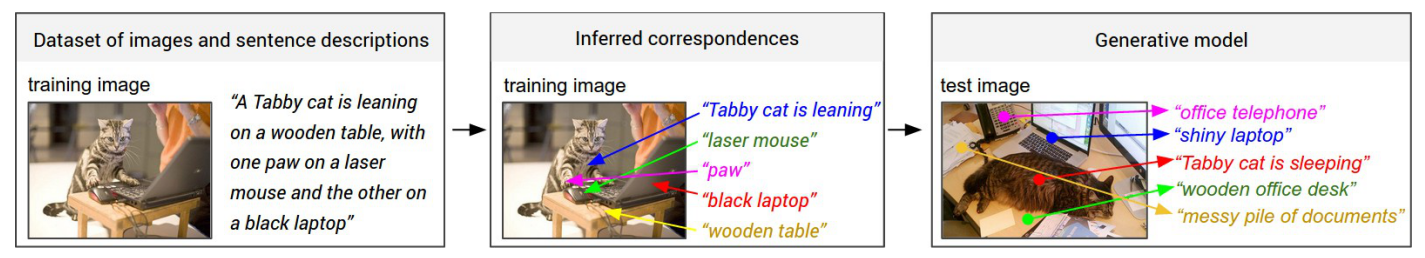
\includegraphics[width=0.8\linewidth]{p2.jpg}
\end{center}
   \caption{Overview of our approach. A dataset of images and their sentence descriptions is the input to our model(left). Our model first infers the correspondences and then learns to generate novel descriptions.}
\label{fig:circle}
\end{figure}

\subsection{Learning to align visual and language data}

Our alignment model assumes an input dataset of images and their sentence descriptions. Our key insight is that sentences written by people make frequent references to some particular, but unknown location in the image. For example, in Figure 2, the words ``Tabby cat is leaning'' refer to the cat, the words ``wooden table'' refer to the table, etc. We would like to infer these latent correspondences, with the eventual goal of later learning to generate these snippets from image regions. We build on the approach of learning to ground dependency tree relations to image regions with a ranking objective. Our contribution is in the use of bidirectional recurrent neural network to compute word representations in the sentence, dispensing of the need to compute dependency trees and allowing unbounded interactions of words and their context in the sentence. We also substantially simplify their objective and show that both modifications improve ranking performance.

We first describe neural networks that map words and image regions into a common, multimodal embedding. Then we introduce our objective, which learns the embedding representations so that semantically similar concepts across the two modalities occupy nearby regions of the space.

{\bf Representing images} We observe that sentence descriptions make frequent references to objects and their attributes. Thus, we follow the method of Girshick et al. [4] to detect objects in every image with a Region Convolutional Neural Network (RCNN). The CNN is pre-trained on ImageNet [6] and finetuned on the 200 classes of the ImageNet Detection Challenge [45]. Following Karpathy et al. [5], we use the top 19 detected locations in addition to the whole image and compute the representations based on the pixels Ib inside each bounding box as follows:

\[v={{W}_{m}}[CN{{N}_{{{\theta }_{c}}}}({{I}_{b}})]+{{b}_{m}}\]

where $CNN(I_b)$ transforms the pixels inside bounding box $I_b$  into 4096-dimensional activations of the fully connected layer immediately before the classifier. The CNN parameters ${\theta }_{c}$ contain approximately 60 million parameters. The matrix $W_m$  has dimensions $h\times 4096$,  where $h$ is the size of the multimodal embedding space ($h$ ranges from $1000- 1600$ in our experiments). Every image is thus represented as a set of h-dimensional vectors $\{{{v}_{i}}|i=1,...,20\}$ .

{\bf Representing sentences}  To establish the inter-modal relationships, we would like to represent the words in the sentence in the same h- dimensional embedding space that the image regions occupy. The simplest approach might be to project every individual word directly into this embedding. However, this approach does not consider any ordering and word context information in the sentence.  An extension to this idea is  to use word bigrams, or dependency tree relations as previously proposed [5]. However, this still imposes an arbitrary maximum size of the context window and requires the use of Dependency Tree Parsers that might be trained on unrelated text corpora.

To address these concerns, we propose to use a Bidirectional Recurrent Neural Network (BRNN) [11] to compute the word representations.

\begin{align}
  & {{x}_{t}}={{W}_{w}}{{I}_{t}} \\ 
 & {{e}_{t}}=f({{W}_{e}}{{x}_{t}}+{{b}_{e}}) \\ 
 & h_{t}^{f}=f({{e}_{t}}+{{W}_{f}}h_{t-1}^{f}+{{b}_{f}}) \\ 
 & h_{t}^{b}=f({{e}_{t}}+{{W}_{b}}h_{t+1}^{b}+{{b}_{b}}) \\ 
 & {{s}_{t}}=f({{W}_{d}}(h_{t}^{f}+h_{t}^{b})+{{b}_{d}}) 
\end{align}

Here, $I_t$ is an indicator column vector that has a single one at the index of the $t$-th word in a word vocabulary. The weights $W_w$ specify a word embedding matrix that we initialize with 300-dimensional word2vec [8] weights and keep fixed due to overfitting concerns. However, in practice we find little change in final performance when these vectors are trained, even from random initialization. Note that the BRNN consists of two independent streams of processing, one moving left to right ($ h_{t}^{f}$ ) and the other right to left ($h_{t}^{b}$) (see Figure 3 for diagram). The final $h$-dimensional representation $s_t$ for the $t$-th word is a function of both the word at that location and also its surrounding context in the sentence. Technically, every $s_t$ is a function of all words in the entire sentence, but our empirical finding is that the final word representations (st) align most strongly to the visual concept of the word at that location ($I_t$).
We learn the parameters $W_e$, $W_f$ , $W_b$, $W_d$ and the respective biases $b_e, b_f , b_b, b_d$.  A typical size of the hidden rep- resentation in our experiments ranges between 300-600 dimensions. We set the activation function $f$ to the rectified
linear unit (ReLU), which computes $f:x\to \max (0,x)$.

\begin{figure}[t]
\begin{center}
%\fbox{\rule{0pt}{2in} \rule{0.9\linewidth}{0pt}}
   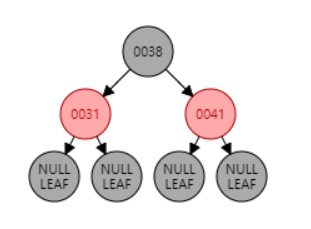
\includegraphics[width=0.8\linewidth]{3.png}
\end{center}
   \caption{Diagram for evaluating the image-sentence score $S_{kl}$. Object regions are embedded with a CNN (left). Words (enriched by their context) are embedded in the same multimodal space with a BRNN(right). Pairwise similarities are computed with inner products (magnitudes shown in grayscale) and finally reduced to image-sentence score}
\label{fig:circle}
\end{figure}

{\bf Alignment objective} We have described the transformations that map every im- age and sentence into a set of vectors in a common h- dimensional space. Since the supervision is at the level of entire images and sentences, our strategy is to formulate an image-sentence score as a function of the individual region- word scores. Intuitively, a sentence-image pair should have a high matching score if its words have a confident support in the image. The objective encourages aligned image-sentences pairs to have a higher score, which is shown as follows:

\begin{align}
  & {{S}_{kl}}=\sum\limits_{t\in {{g}_{l}}}{\sum\limits_{i\in {{g}_{k}}}{\max (0,v_{i}^{T}{{s}_{t}})}} \\ 
 & C(\theta )=\sum\limits_{k}{[\sum\limits_{l}{\max (0,{{S}_{kl}}-{{S}_{kk}}+1)+\sum\limits_{l}{\max (0,{{S}_{lk}}-{{S}_{kk}}+1)}}]}  
\end{align}

Where $g_k$  is the set of image fragments in image $k$  and $g_l$  is the set of sentence fragments in sentence $l$. The indices $k, l$ range over the images and sentences in the training set. Together with their additional Multiple Instance Learning objective, this score carries the interpretation that a sentence fragment aligns to a subset of the image regions whenever the dot product is positive. $C(\theta )$ denotes the structured loss. 



\subsection{Multimodal Recurrent Neural Network for generating descriptions}

In this section we assume an input set of images and their textual descriptions. These could be full images and their sentence descriptions, or regions and text snippets, as inferred in the previous section. The key challenge is in the design of a model that can predict a variable-sized sequence of outputs given an image. In previously developed language models based on Recurrent Neural Networks (RNNs) [13], this is achieved by defining a probability distri bution of the next word in a sequence given the current word and context from previous time steps. We explore a simple but effective extension that additionally conditions the generative process on the content of an input image. More for mally, during training our Multimodal RNN takes the image pixels $I$ and a sequence of input vectors $(x_1, . . . , x_T )$. It then computes a sequence of hidden states ($h_1, . . . , h_t$) and a sequence of outputs ($y_1, . . . , y_t$) by iterating the following recurrence relation for $t = 1$ to $T$ : 

\begin{align}
  & {{b}_{v}}={{W}_{hi}}[CN{{N}_{{{\theta }_{c}}}}(I)] \\ 
 & {{h}_{t}}=f({{W}_{hx}}{{x}_{t}}+{{W}_{hh}}{{h}_{t-1}}+{{b}_{h}}+I(t=1)\odot {{b}_{v}}) \\ 
 & {{y}_{t}}=soft\max ({{W}_{oh}}{{h}_{t}}+{{b}_{o}}) 
\end{align}

Where $W_{hi}, W_{hx}, W_{hh}, W_{oh}, x_i$ and $b_h, b_o$ are learnable parameters, and $CN{{N}_{{{\theta }_{c}}}}(I)$ is the last layer of a CNN. The output vector $y_t$ holds the (unnormalized) log probabilities of words in the dictionary and one additional dimension for a special END token. Note that we provide the image context vector $b_v$ to the RNN only at the first iteration, which we found to work better than at each time step. In practice we also found that it can help to also pass both $b_v$, ($W_{hx}x_t$) through the activation function. A typical size of the hidden layer of the RNN is 512 neurons.

{\bf RNN training}. The RNN is trained to combine a word ($x_t$), the previous context ($h_{t−1}$) to predict the next word ($y_t$). We condition the RNN’s predictions on the image information ($b_v$) via bias interactions on the first step. The training proceeds as follows (refer to Figure 4): We set  $h_0 = 0$, $x_1$ to a special START vector, and the desired label $y_1$ as the first word in the sequence. Analogously, we set $x_2$ to the word vector of the first word and expect the network to predict the second word, etc. Finally, on the last step when $x_T$ represents the last word, the target label is set to a special END token. The cost function is to maximize the log probability assigned to the target labels (i.e. Softmax classifier).

\begin{figure}[t]
\begin{center}
%\fbox{\rule{0pt}{2in} \rule{0.9\linewidth}{0pt}}
   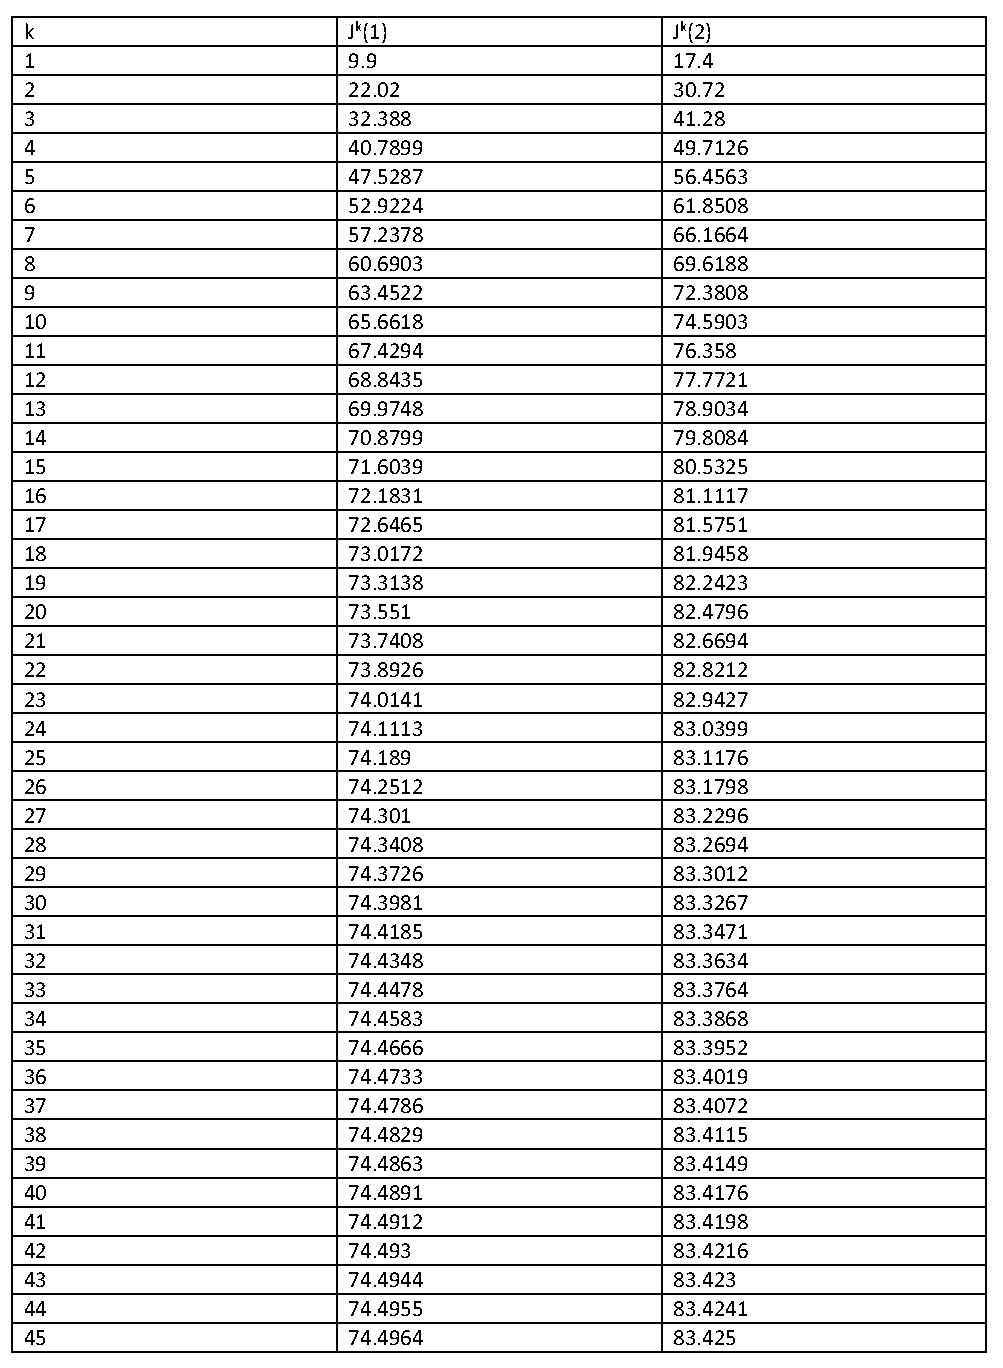
\includegraphics[width=0.8\linewidth]{44.png}
\end{center}
   \caption{Image-Sentence ranking experiments results.  Med r is the median rank(low is good)}
\label{fig:circle}
\end{figure}

\begin{figure}[t]
\begin{center}
%\fbox{\rule{0pt}{2in} \rule{0.9\linewidth}{0pt}}
   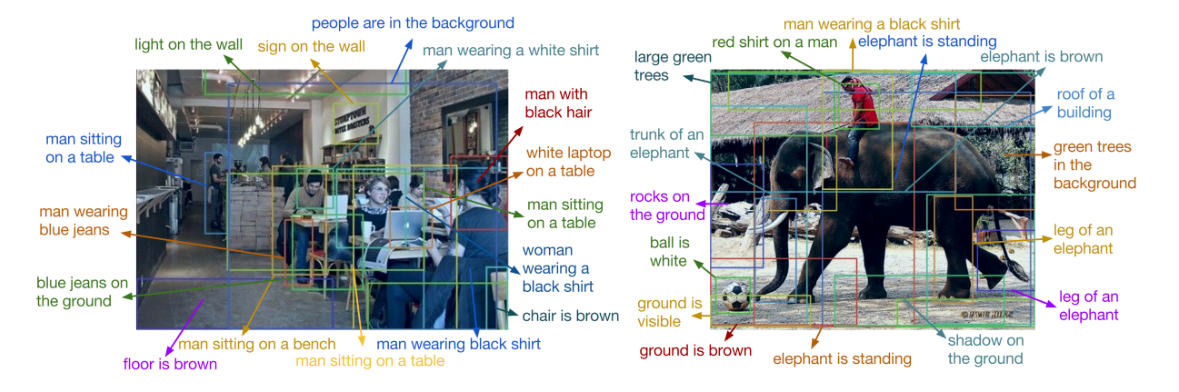
\includegraphics[width=0.8\linewidth]{j22.jpg}
\end{center}
   \caption{Example alignments predicted by our model.}
\label{fig:circle}
\end{figure}


\begin{figure}[t]
\begin{center}
%\fbox{\rule{0pt}{2in} \rule{0.9\linewidth}{0pt}}
   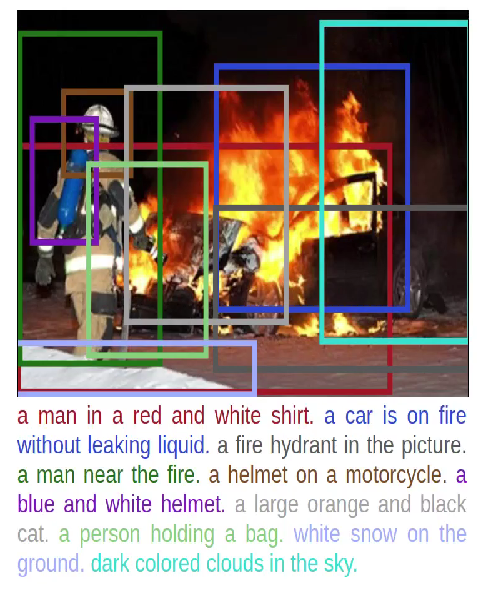
\includegraphics[width=0.8\linewidth]{j23.jpg}
\end{center}
   \caption{Example sentences generated by the multimodal RNN for test images.}
\label{fig:circle}
\end{figure}

\begin{figure}[t]
\begin{center}
%\fbox{\rule{0pt}{2in} \rule{0.9\linewidth}{0pt}}
   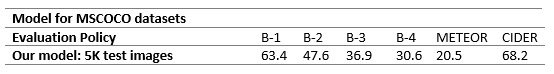
\includegraphics[width=0.8\linewidth]{61.png}
\end{center}
   \caption{Evaluation of full image predictions on 5,000 test images. B-n is BLEU score that uses up to n-grams. High is good in all columns. }
\label{fig:circle}
\end{figure}

\section{Performance Results}

{\bf Datasets} In this project, We use 
MSCOCO [7] datasets in our experiments. These datasets
contain 123,000 images 
and each is annotated with 5 sentences using Amazon
Mechanical Turk.  we
use 5,000 images for both validation and testing.\\
{\bf Data Preprocessing} We convert all sentences to lower- case, discard non-alphanumeric characters. We filter words to those that occur at least 5 times in the training set, which results in  8791 words for MSCOCO datasets.


\subsection{Image-Sentence Alignment Evaluation}

We first investigate the quality of the inferred text and image alignments with ranking experiments. We consider a withheld set of images and sentences and retrieve items in one modality given a query from the other by sorting based on the image-sentence score $S_{kl}$. We report the median rank of the closest ground truth result in the list, which measures the fraction of times a correct item was found among the top K results. The result of these experiments can be found in Figure 4, and example retrievals in Figure 5. We now highlight some of the takeaways.





\subsection{Generated Descriptions: Fulframe evaluation}

We now evaluate the ability of our RNN model to describe images and regions. We first trained our Multimodal RNN to generate sentences on full images with the goal of verifying that the model is rich enough to support the mapping from image data to sequences of words. For these full image experiments we use the more powerful VGGNet image features [12]. We report the BLEU [9], METEOR [2] and CIDEr  [14]  scores  computed  with  the coco-caption
code.  Each method evaluates a candidate sentence
by measuring how well it matches a set of five reference
sentences written by humans.

Figure 6 and figure 7 show that the Multimodal RNN confidently outperforms this retrieval method. Hence, even with 113,000 train set images in MSCOCO the retrieval approach is inadequate. Additionally, the RNN takes only a fraction of a second to evaluate per image.





\section{Conclusion}

We introduced a model that generates natural language descriptions of image regions based on weak labels in form of a dataset of images and sentences, and with very few hard- coded assumptions. Our approach features a novel ranking model that aligned parts of visual and language modalities through a common, multimodal embedding. We showed that this model provides state of the art performance on image-sentence ranking experiments. Second, we described a Multimodal Recurrent Neural Network architecture that generates descriptions of visual data. We evaluated its performance on both fullframe and region-level experiments and showed that in both cases the Multimodal RNN outperforms retrieval baselines.

\section{Reference}
%\begin{thebibliography}{9}
%\bibitem{latexcompanion} 
%Michel Goossens, Frank Mittelbach, and Alexander Samarin. 
%\textit{The \LaTeX\ Companion}. 
%Addison-Wesley, Reading, Massachusetts, 1993.
% 
%\bibitem{einstein} 
%Albert Einstein. 
%\textit{Zur Elektrodynamik bewegter K{\"o}rper}. (German) 
%[\textit{On the electrodynamics of moving bodies}]. 
%Annalen der Physik, 322(10):891–921, 1905.
% 
%\bibitem{knnnuthwebsite} 
%Knuth: Computers and Typesetting,
%\\\texttt{http://www-cs-faculty.stanford.edu/\~{}uno/abcde.html}
%
%\bibitem{einstein} 
%Y. Bengio,  H. Schwenk,  J.-S. Sen  e´cal,  F. Morin,  and J.-L. Gauvain 
%\textit{Neural probabilistic language models}.  
%In Innova- tions in Machine Learning. Springer, 2006.
%
%\bibitem{einstein} 
%Y. Bengio,  H. Schwenk,  J.-S. Sen  e´cal,  F. Morin,  and J.-L. Gauvain 
%\textit{Neural probabilistic language models}.  
%In Innova- tions in Machine Learning. Springer, 2006.
%
%\bibitem{einstein} 
%K. Barnard, P. Duygulu, D. Forsyth, N. De Freitas, D. M. Blei, and M. I. Jordan 
%\textit{Matching words and pictures}.  
%JMLR, 2003.
%
%\bibitem{einstein} 
%X.  Chen  and  C.  L.  Zitnick 
%\textit{Matching words and pictures}.  
% CoRR, abs/1411.5654, 2014
%
%\bibitem{einstein} 
%J. Deng, W. Dong, R. Socher, L.-J. Li,  K. Li,  and L. Fei- Fei
%\textit{Imagenet: A large-scale hierarchical image database}.  
%In CVPR, 2009.
%
%\bibitem{einstein} 
%J. Donahue, L. A. Hendricks, S. Guadarrama, M. Rohrbach,
%S. Venugopalan, K. Saenko, and T. Darrell
%\textit{Long-term recur- rent convolutional networks for visual recognition and de- scription.}.  
%arXiv preprint arXiv:1411.4389, 2014.
%
%[11]M. Everingham, L. Van Gool, C. K. I. Williams, J. Winn, and
%A. Zisserman. The pascal visual object classes (voc) chal- lenge. International Journal of Computer Vision, 88(2):303– 338, June %2010.\\
%[1]A. Barbu, A. Bridge, Z. Burchill, D. Coroian, S. Dickin-  son, S. Fidler, A. Michaux, S. Mussman, S. Narayanaswamy,
%D. Salvi, et al. Video in sentences out. arXiv preprint arXiv:1204.2742, 2012. \\
%
%[2]K. Barnard, P. Duygulu, D. Forsyth, N. De Freitas, D. M. Blei, and M. I. Jordan. Matching words and pictures. JMLR, 2003. \\
%
%[3]Y. Bengio,  H. Schwenk,  J.-S. Sen  e´cal,  F. Morin,  and J.-L. Gauvain. Neural probabilistic language models. In Innova- tions in Machine Learning. Springer, 2006.\\
%
%[4]X. Chen, H. Fang, T.-Y. Lin, R. Vedantam, S. Gupta, P. Dol- lar, and C. L. Zitnick. Microsoft coco captions: Data collec- tion and evaluation server. arXiv preprint arXiv:1504.00325, 2015.\\
%
%[5]X.  Chen  and  C.  L.  Zitnick.	Learning a recurrent vi- sual representation for image caption generation. CoRR, abs/1411.5654, 2014.\\

[1]J. Deng, W. Dong, R. Socher, L.-J. Li,  K. Li,  and L. Fei- Fei. Imagenet: A large-scale hierarchical image database. In CVPR, 2009.\\

[2]M. Denkowski and A. Lavie. Meteor universal: Language specific translation evaluation for any target language. In Proceedings of the EACL 2014 Workshop on Statistical Ma- chine Translation, 2014.\\

%[8]J. Donahue, L. A. Hendricks, S. Guadarrama, M. Rohrbach,
%S. Venugopalan, K. Saenko, and T. Darrell. Long-term recur- rent convolutional networks for visual recognition and de- scription. arXiv preprint arXiv:1411.4389, 2014.\\
%
%[9]D. Elliott and F. Keller. Image description using visual de- pendency representations. In EMNLP, pages 1292–1302, 2013.\\
%
%[10]J. L. Elman.   Finding structure in time.	Cognitive science, 14(2):179–211, 1990.\\
%
%[11]M. Everingham, L. Van Gool, C. K. I. Williams, J. Winn, and
%A. Zisserman. The pascal visual object classes (voc) chal- lenge. International Journal of Computer Vision, 88(2):303– 338, June 2010.\\
%
%[12]H. Fang, S. Gupta, F. Iandola, R. Srivastava, L. Deng,
%P.  Dolla´r,   J.  Gao,   X.  He,   M.  Mitchell,   J.  Platt,   et  al. From captions to visual concepts and back. arXiv preprint arXiv:1411.4952, 2014.\\
%
%[13]A. Farhadi, M. Hejrati, M. A. Sadeghi, P. Young,
%C. Rashtchian, J. Hockenmaier, and D. Forsyth. Every pic- ture tells a story: Generating sentences from images. In ECCV. 2010.\\

[3]L. Fei-Fei, A. Iyer, C. Koch, and P. Perona. What do we perceive in a glance of a real-world scene? Journal of vision, 7(1):10, 2007.\\

%[15]S. Fidler, A. Sharma, and R. Urtasun. A sentence is worth a thousand pixels. In CVPR, 2013.\\
%
%[16]A. Frome, G. S. Corrado, J. Shlens, S. Bengio, J. Dean,
%T. Mikolov, et al. Devise: A deep visual-semantic embed- ding model. In NIPS, 2013.\\

[4]R. Girshick, J. Donahue, T. Darrell, and J. Malik. Rich fea- ture hierarchies for accurate object detection and semantic segmentation. In CVPR, 2014.\\


%[18]S. Gould, R. Fulton, and D. Koller. Decomposing a scene into geometric and semantically consistent regions. In Com- puter Vision, 2009 IEEE 12th International Conference on, pages 1–8. IEEE, 2009.\\
%
%[19]A. Gupta and P. Mannem.  From image annotation to im-  age description. In Neural information processing. Springer, 2012.\\
%
%[20]S. Hochreiter and J. Schmidhuber. Long short-term memory.
%Neural computation, 9(8):1735–1780, 1997.\\
%
%[21]M. Hodosh, P. Young, and J. Hockenmaier. Framing image description as a ranking task: data, models and evaluation metrics. Journal of Artificial Intelligence Research, 2013.\\
%
%[22]R. JeffreyPennington and C. Manning. Glove: Global vec- tors for word representation. 2014.\\
%
%[23]Y. Jia, M. Salzmann, and T. Darrell. Learning cross-modality similarity for multinomial data. In ICCV, 2011.\\

[5]A. Karpathy, A. Joulin, and L. Fei-Fei. Deep fragment em- beddings for bidirectional image sentence mapping. arXiv preprint arXiv:1406.5679, 2014.\\

%[25]R. Kiros, R. Salakhutdinov, and R. S. Zemel. Unifying visual-semantic embeddings with multimodal neural lan- guage models. arXiv preprint arXiv:1411.2539, 2014.\\
%
%[26]R. Kiros, R. S. Zemel, and R. Salakhutdinov. Multimodal neural language models. ICML, 2014.\\
%
%[27]C. Kong, D. Lin, M. Bansal, R. Urtasun, and S. Fidler. What are you talking about? text-to-image coreference. In CVPR, 2014.\\
%
%[28]A. Krizhevsky, I. Sutskever, and G. E. Hinton. Imagenet classification with deep convolutional neural networks. In NIPS, 2012.\\

[6]G. Kulkarni, V. Premraj, S. Dhar, S. Li, Y. Choi, A. C. Berg, and T. L. Berg. Baby talk: Understanding and generating simple image descriptions. In CVPR, 2011.\\

%[30]P. Kuznetsova, V. Ordonez, A. C. Berg, T. L. Berg, and
%Y. Choi. Collective generation of natural image descriptions. In ACL, 2012.\\
%
%[31]P. Kuznetsova, V. Ordonez, T. L. Berg, U. C. Hill, and
%Y. Choi. Treetalk: Composition and compression of trees for image descriptions. Transactions of the Association for Computational Linguistics, 2(10):351–362, 2014.\\
%
%[32]Y. LeCun, L. Bottou, Y. Bengio, and P. Haffner. Gradient- based learning applied to document recognition. Proceed- ings of the IEEE, 86(11):2278–2324, 1998.\\
%
%[33]L.-J. Li and L. Fei-Fei. What, where and who? classifying events by scene and object recognition. In ICCV, 2007.\\
%
%[34]L.-J. Li, R. Socher, and L. Fei-Fei. Towards total scene un- derstanding: Classification, annotation and segmentation in an automatic framework. In Computer Vision and Pattern Recognition, 2009. CVPR 2009. IEEE Conference on, pages 2036–2043. IEEE, 2009.\\
%
%[35]S. Li, G. Kulkarni, T. L. Berg, A. C. Berg, and Y. Choi. Com- posing simple image descriptions using web-scale n-grams. In CoNLL, 2011.\\
%
%[36]D. Lin, S. Fidler, C. Kong, and R. Urtasun. Visual semantic search: Retrieving videos via complex textual queries. 2014.\\

[7]T.-Y. Lin, M. Maire, S. Belongie, J. Hays, P. Perona, D. Ra- manan, P. Dolla´r, and C. L. Zitnick.  Microsoft coco:  Com- mon objects in context. arXiv preprint arXiv:1405.0312,2014.\\

%[38]J. Mao, W. Xu, Y. Yang, J. Wang, and A. L. Yuille. Explain images with multimodal recurrent neural networks. arXiv preprint arXiv:1410.1090, 2014.\\
%
%[39]C. Matuszek*, N. FitzGerald*, L. Zettlemoyer, L. Bo, and
%D. Fox. A Joint Model of Language and Perception for Grounded Attribute Learning. In Proc. of the 2012 Interna- tional Conference on Machine Learning, Edinburgh, Scot- land, June 2012.\\
%
%[40]T. Mikolov, M. Karafi  a´t, L. Burget, J. Cernocky`, and S. Khu- danpur. Recurrent neural network based language model. In INTERSPEECH, 2010.\\

[8]T. Mikolov, I. Sutskever, K. Chen, G. S. Corrado, and
J. Dean. Distributed representations of words and phrases and their compositionality. In NIPS, 2013.\\

%[42]M. Mitchell, X. Han, J. Dodge, A. Mensch, A. Goyal,
%A. Berg, K. Yamaguchi, T. Berg, K. Stratos, and H. Daume´,
%III. Midge: Generating image descriptions from computer vision detections. In EACL, 2012.\\
%
%[43]V. Ordonez, G. Kulkarni, and T. L. Berg. Im2text: Describ- ing images using 1 million captioned photographs. In NIPS, 2011.\\

[9]K. Papineni, S. Roukos, T. Ward, and W.-J. Zhu. Bleu: a method for automatic evaluation of machine translation. In Proceedings of the 40th annual meeting on association for computational linguistics, pages 311–318. Association for Computational Linguistics, 2002.\\

[10]O. Russakovsky, J. Deng, H. Su, J. Krause, S. Satheesh,
S. Ma, Z. Huang, A. Karpathy, A. Khosla, M. Bernstein,
A. C. Berg, and L. Fei-Fei. Imagenet large scale visual recog- nition challenge, 2014.\\

[11]M. Schuster and K. K. Paliwal. Bidirectional recurrent neural networks. Signal Processing, IEEE Transactions on, 1997. [47]K. Simonyan and A. Zisserman. Very deep convolutional
networks for large-scale image recognition. arXiv preprint
arXiv:1409.1556, 2014.\\


[12]K. Simonyan and A. Zisserman. Very deep convolutional
networks for large-scale image recognition. arXiv preprint
arXiv:1409.1556, 2014.
%[48]R. Socher and L. Fei-Fei. Connecting modalities: Semi- supervised segmentation and annotation of images using un- aligned text corpora. In CVPR, 2010.\\
%
%[49]R. Socher, A. Karpathy, Q. V. Le, C. D. Manning, and A. Y. Ng. Grounded compositional semantics for finding and de- scribing images with sentences. TACL, 2014.\\

[13]I. Sutskever, J. Martens, and G. E. Hinton. Generating text with recurrent neural networks. In ICML, 2011.\\

%[51]C. Szegedy, W. Liu, Y. Jia, P. Sermanet, S. Reed,
%D. Anguelov, D. Erhan, V. Vanhoucke, and A. Rabi- novich. Going deeper with convolutions. arXiv preprint arXiv:1409.4842, 2014.\\
%
%[52]T. Tieleman and G. E. Hinton. Lecture 6.5-rmsprop: Divide the gradient by a running average of its recent magnitude., 2012.\\

[14]R.   Vedantam,   C.   L.   Zitnick,   and D.  Parikh.	Cider: Consensus-based  image  description  evaluation.		CoRR, abs/1411.5726, 2014.\\


%[54]O. Vinyals, A. Toshev, S.  Bengio,  and  D.  Erhan.  Show and tell: A neural image caption generator. arXiv preprint arXiv:1411.4555, 2014.\\
%
%[55]Y. Yang, C. L. Teo, H. Daum e´III, and Y. Aloimonos.
%Corpus-guided sentence generation of natural images. In
%EMNLP, 2011.\\
%
%[56]B. Z. Yao, X. Yang, L. Lin, M. W. Lee, and S.-C. Zhu. I2t: Image parsing to text description. Proceedings of the IEEE, 98(8):1485–1508, 2010.\\
%
%[57]M. Yatskar, L. Vanderwende, and L. Zettlemoyer. See no evil, say no evil: Description generation from densely la- beled images. Lexical and Computational Semantics, 2014.\\
%
%[58]P. Young, A. Lai, M. Hodosh, and J. Hockenmaier. From im- age descriptions to visual denotations: New similarity met- rics for semantic inference over event descriptions. TACL, 2014.\\
%
%[59]W. Zaremba, I. Sutskever, and O. Vinyals.  Recurrent neu- ral network regularization. arXiv preprint arXiv:1409.2329, 2014.\\
%
%[60]C. L. Zitnick, D. Parikh, and L. Vanderwende. Learning the visual interpretation of sentences. ICCV, 2013.\\






%\end{thebibliography}

\section{Appendix A: Explanation of Files Used in this Project}

The appendix A is shown in Figure 8.

\begin{figure}[t]
\begin{center}
%\fbox{\rule{0pt}{2in} \rule{0.9\linewidth}{0pt}}
   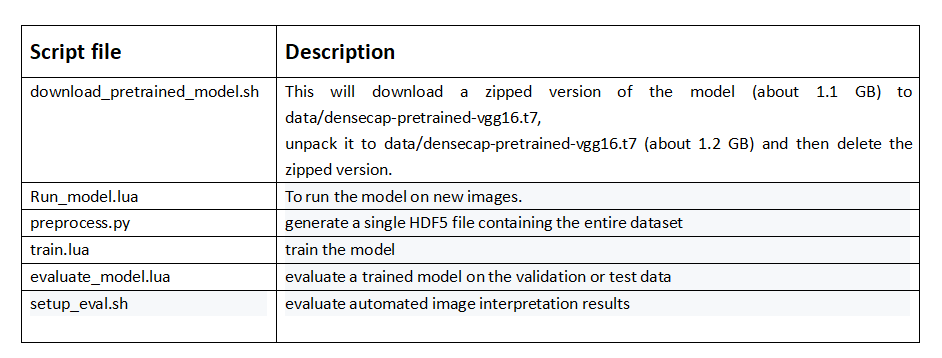
\includegraphics[width=0.8\linewidth]{ap1.jpg}
\end{center}
   \caption{Listing of Project Files }
\label{fig:circle}
\end{figure}











\end{document}









